\chapter{Reducibility}

\section{The Reducibility Method}
If we know that some problem (say \(A_{TM}\)) is undecidable, we can use that to show other problems are undecidable.

\begin{remark}
    Review the proof of HALT problem.
\end{remark}

\begin{definition}[Reducibility]
    If we have 2 languages (or problems) \(A\) and \(B\), then \(A\) is reducible to \(B\) means that we can use \(B\) to solve \(A\).  
\end{definition}

\begin{example}
    Measuring the area of a rectangle is reducible to measuring the lengths of its sides.
\end{example}

\begin{example}
    We showed that \(A_{NFA}\) is reducible to \(A_{DFA}\). 
\end{example}


If \(A\) is reducible to \(B\) then solving \(B\) gives a solution to \(A\):
\begin{itemize}
    \item then \(B\) is easy \(\rightarrow\) \(A\) is easy.   
    \item \fbox{then \(A\) is hard \(\rightarrow\) \(B\) is hard.}  (this is the form we will use) 
\end{itemize}  


\section{General Reducibility}

\begin{theorem}
    Let \(E_{TM}\) = \{ \(\langle M \rangle\) | \(M\) is a TM and \(L(M) = \emptyset\) \}

    \(E_{TM}\) is undecidable. 
\end{theorem}
\begin{proof}
    Proof by contradiction. Show that \(A_{TM}\) is reducible to \(E_{TM}\).  

    Assume that \(E_{TM}\) is decidable and show that \(A_{TM}\) is decidable.  

    Let TM R decide \(E_{TM}\) 

    Construct TM S deciding \(A_{TM}\) 

    \begin{remark}
        A naive idea will be constructing \(S\) to run \(R\) on \(\langle M \rangle\). 
        But here is the problem, if \(R\) accepts \(\langle M \rangle\), meaning \(M\) accepts no string, that is \(L(M) = \emptyset\), this is good.    
        But if \(R\) reject \(\langle M \rangle\), we know \(M\) must accept some language, but we don't know what language.   
        
        That's why we need a modified \(M\). 
    \end{remark}

    \(S\) = "On input \(\langle M, w \rangle\) 
    \begin{enumerate}
        \item We can use \(M\) and \(w\) to construct a TM \(M_w\). 

        \(M_w\) = "On input \(x\)
        \begin{enumerate}
            \item If \(x \neq w\), reject
            \item If \(x \neq w\), run \(M\) on input \(w\) and accept if \(M\) does."
        \end{enumerate}  

        \item Run \(R\) on input \(\langle M_w \rangle\)
        \item If \(R\) accepts, \(reject\); if \(R\) rejects, \(accept\)."      
    \end{enumerate}
\end{proof}

\section{Mapping Reducibility}

\begin{definition}
    A function \(f: \Sigma^* \rightarrow \Sigma^*\) is a \underline{computable function} if there is a TM \(F\) where \(F\) on input \(w\) halts with \(f(w)\) on its tape for all strings \(w\).     
    \begin{note}[rephrase]
        \(f: \Sigma^* \rightarrow \Sigma^*\)  is \textbf{ computable (or Turing computable)} if there is some TM \(M\) and for all \(w\), \(M\) will take \(w\) as input, and write \(f(w)\) on the tape.      
    \end{note}
\end{definition}

\begin{example}
    Arithmetic operations on integers are computable functions.

    For example, we can make a machine that takes input \(\langle m, n \rangle\) and returns \(m + n\). 
\end{example}

\begin{definition}
    \underline{\(A\) is mapping-reducible to \(B\)}(\(A \leq_m B\)) \textbf{if there is} a computable function \(f\) where \(w \in A\) iff \(f(w) \in B\).   

    \begin{figure}[H]
        \centering
        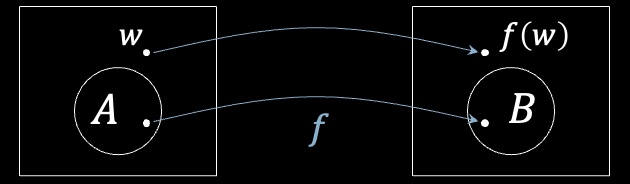
\includegraphics[width=0.8\textwidth]{l9.1.jpg}
        \caption{Function \(f\) reducing \(A\) to \(B\)}
    \end{figure}
\end{definition}

\begin{example}\label{example: 9.1}
    \(A_{TM} \leq_m \overline{E_{TM}}\)     

    The computable reduction function \(f\) is \(f(\langle M, w \rangle) = \langle M_w \rangle\) 

    \begin{remark}
        Recall TM \(M_w\)  = "On input x
        \begin{enumerate}
            \item if \(x \neq w\), reject
            \item else run \(M\) on w
            \item Accept if M accepts"  
        \end{enumerate}
    \end{remark}

    Because \(\langle M, w\rangle \in A_{TM} \) iff \(\langle M_w \rangle \in \overline{E_{TM}}\) (M accepts w iff \(L(\langle M_w \rangle) \neq \emptyset\))  
\end{example}

\subsection{Mapping Reductions - properties}

\begin{theorem}
    If \(A \leq_m B\) and \(B\) is decidable then so is \(A\)   
\end{theorem}
The theorem means there is a computable function (reduction function) which takes any input and produces an output where the input in \(A\) iff the output is in \(B\).  
\begin{proof}
    Say TM R decides B.

    Construct TM S deciding A:
    S = "On input w
    \begin{enumerate}
        \item Compute \(f(w)\)
        \item Run \(R\) on \(f(w)\) to test if \(f(w) \in B\) 
        \begin{remark}
            Because R decides B, then \(R\) is a decider. A TM is a decider means this TM will halt on every input, no matter if the input is in B. 
        \end{remark}
        \item If \(R\) halts then output the same result."
    \end{enumerate}
\end{proof}
\begin{remark}
    According to this theorem, we can conclude that for \hyperref[example: 9.1]{this example}, if \(\overline{E_{TM}}\) is decidable, then \(A_{TM}\) is decidable.  
    Because we all know that \(A_{TM}\) is not decidable, so \(\overline{E_{TM}}\) is not decidable.  
\end{remark}


\begin{corollary}
    If \(A \leq_m B\) and \(A\) is undecidable then so is \(B\)   
\end{corollary}

\begin{theorem}
    If \(A \leq_m B\) and \(B\) is T-recognizable then so is \(A\).   
\end{theorem}
\begin{proof}
    Same as above    
\end{proof}

\begin{corollary}
    If \(A \leq_m B\) and \(A\) is T-unrecognizable then so is B. 
\end{corollary}

\begin{theorem}
    \(A \leq_m B \iff \overline{A} \leq_m \overline{B}\)  
\end{theorem}
\begin{proof}
    This is because \(A \leq_m B\)  implies if there is an x in A, iff \(f(x)\) is in B.  

    So if x not in \(A\), only if \(f(x)\) is not in B. Which is the complement form.  
\end{proof}
\begin{corollary}
    For the same reason, we know that \(A_{TM} \not\leq_m E_{TM}\), so we can say \(\overline{A_{TM}} \not\leq \overline{E_{TM}}\).  
\end{corollary}

\subsection{Mapping vs General Reducibility}
They are not the same!

\subsubsection{Mapping Reducibility of \(A\) to \(B\): Translate A-questions to B-questions}
\begin{figure}[H]
        \centering
        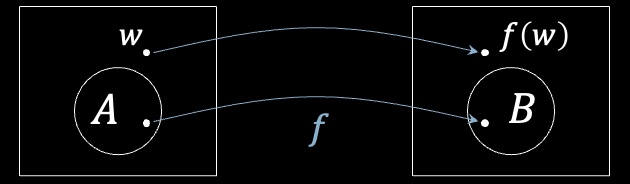
\includegraphics[width=0.6\textwidth]{l9.1.jpg}
        \caption{Showing Mapping Reducibility}
\end{figure}
\begin{itemize}
    \item A special type of reducibility.
    \item Useful to prove T-unrecognizability.
\end{itemize}

\subsubsection{(General) Reducibility of \(A\) to \(B\): Use \(B\) solver to solve \(A\)}
\begin{figure}[H]
        \centering
        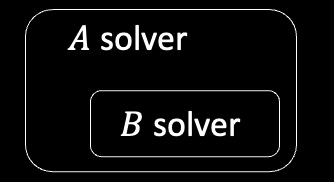
\includegraphics[width=0.4\textwidth]{l9.2.jpg}
        \caption{Showing General Reducibility}
\end{figure}
\begin{itemize}
    \item May be conceptually simpler
    \item Useful to prove Undecidability
\end{itemize}

\subsubsection{Noteworthy difference:} 
\begin{enumerate}
    \item \(A\) is reducible to \(\overline{A}\)  
    \item \(A\) may not be mapping reducible to \(\overline{A}\)  
    \begin{example}
        \(
        \overline{A_{TM}} \not\leq_m A_{TM}
        \) 
    \end{example}
\end{enumerate}


\subsection{Reducibility - Templates}

\subsubsection{To prove \(B\) is undecidable:} 
\begin{itemize}
    \item Show undecidable A is reducible to B (often A is \(A_{TM}\)) 
    \item Template: Assume TM R decides B, Construct TM S deciding A. Contradiction.
\end{itemize}

\subsubsection{To prove \(B\) is T-unrecognizable:} 
\begin{itemize}
    \item Show T-unrecognizable A is mapping reducible to B. (often \(A\) is \(\overline{A_{TM}}\)).
    \item Template: give reduction function \(f\) 
\end{itemize}

\begin{theorem}
    Recall \(E_{TM} = \)\{ \(\langle M \rangle\)| \(M\) is a TM and \(L(M) = \emptyset\)\} 

    \(E_{TM}\) is T-unrecognizable 
\end{theorem}
\begin{proof}
    (We have already shown it is undecidable)    

    Show \(\overline{A_{TM}} \leq_m E_{TM}\) 
    
    Reduction function \(f(\langle M, w \rangle) = \langle M_w \rangle\).
    \begin{remark}
        \(M_w\) is the same machine we have constructed before.
    \end{remark}
\end{proof}


\begin{theorem}
    \(EQ_{TM}\) = \{ \(\langle M_1, M_2 \rangle\)| \(M_1\) and \(M_2\) are TMs and \(L(M_1) = L(M_2)\)  \} 

    Both \(EQ_{TM}\) and \(\overline{EQ_{TM}}\) are T-unrecognizable  
\end{theorem}
\begin{proof}
    \begin{enumerate}
        \item 
        \(
        \overline{A_{TM}} \leq_m EQ_{TM} 
        \) 
        \item
        \(
        \overline{A_{TM}} \leq_m \overline{EQ_{TM}}
        \) 
    \end{enumerate}

    For any \(w\) let \(T_w\) = "On input x
    \begin{enumerate}
        \item ignore x
        \item Simulate M on w"
    \end{enumerate}  

    \begin{enumerate}
        \item \(f(\langle M, w\rangle) = \langle T_w, T_{reject} \rangle\) (\( T_{reject}\) is a TM that always rejects) 
        \item \(f(\langle M, w\rangle) = \langle T_w, T_{accept} \rangle\) (\( T_{accept}\) is a TM that always accepts) 
    \end{enumerate}
\end{proof}

\section{Problems}

\begin{problem}[Rice's theorem]
    Let \(P\) be any nontrivial property of the language of a Turing machine.
    Prove that the problem of determining whether a given Turing machine's language has property \(P\) is undecidable.

    In more formal terms, let \(P\) be a language consisting of Turing machine descriptions where \(P\) fulfills two conditions.  
    First, \(P\) is nontrivial -- it contains some, but not all, TM descriptions.  
    Second, \(P\) is a property of the TM's language -- whenever \(L(M_1) = L(M_2)\), we have \(\langle M_1 \rangle \in P \iff \langle M_2 \rangle \in P\).  
    Here, \(M_1\) and \(M_2\) are any TMs. Prove that \(P\) is an undecidable language.  
\end{problem}
